% ****** Start of file aipsamp.tex ******
%
%   This file is part of the AIP files in the AIP distribution for REVTeX 4.
%   Version 4.1 of REVTeX, October 2009
%
%   Copyright (c) 2009 American Institute of Physics.
%
%   See the AIP README file for restrictions and more information.
%
% TeX'ing this file requires that you have AMS-LaTeX 2.0 installed
% as well as the rest of the prerequisites for REVTeX 4.1
%
% It also requires running BibTeX. The commands are as follows:
%
%  1)  latex  aipsamp
%  2)  bibtex aipsamp
%  3)  latex  aipsamp
%  4)  latex  aipsamp
%
% Use this file as a source of example code for your aip document.
% Use the file aiptemplate.tex as a template for your document.
\documentclass[%
 aip,
 jmp,%
 amsmath,amssymb,
%preprint,%
 reprint,%
%author-year,%
%author-numerical,%
]{revtex4-1}

\usepackage[utf8]{inputenc}
\usepackage{graphicx}% Include figure files
\usepackage{dcolumn}% Align table columns on decimal point
\usepackage{bm}% bold math
%\usepackage[mathlines]{lineno}% Enable numbering of text and display math
%\linenumbers\relax % Commence numbering lines
\usepackage{hyperref}
\usepackage{color}
\usepackage{multirow}

\begin{document}

%\preprint{AIP/123-QED}

\title[Introduction to Machine Learning - Project]{Classification models for protein ligandibility prediction}% Force line breaks with \\

\author{Jakub Bahyl}
\affiliation{%
MFF, NPFL054%\\This line break forced% with \\
}%

\date{\today}% It is always \today, today,
             %  but any date may be explicitly specified

\begin{abstract}
In this work, I'm introducing various automatic predictors, trained on development open dataset of protein points. List of basic applied methods are: \textit{decision tree, random forest, support vector machine} and \textit{logistic regression}. All of them were tuned at it's best and cross-validated on development data.
\end{abstract}

\keywords{proteins, random forest, support vector machines}%Use showkeys class option if keyword
                              %display desired
\maketitle

\begin{quotation}
\textit{"In ML, where algorithms get published quickly and state-of-the-art frameworks are open-source, there isn't any first-mover advantage."\\
— François Chollet}
\end{quotation}



%%%%%%%%%%%%%%%%%%%%%%%%%%%%%%%%%%%%%%%%%%%%%%%%%%%%%%%%%%%%%%%%%%%%%%%%%%%%%%%%%%%
\section*{Intro and Motivation}

Biological functions of proteins are performed by their interaction with other molecules (another proteins, ligands, etc.). Specifically, ligand is an ion or molecule that binds to a central atom to form a coordination complex. Usually there exist several number of points on protein surface with high probability of \textit{ligandibility} - ability to bind a ligand.

\begin{figure}[h]
	\centering

	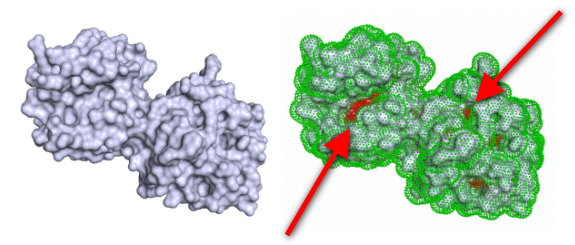
\includegraphics[width=0.5\textwidth]{graphics/proteins.png}

	\caption{On left: Generic protein. On right: Highlighted points with high ligandibility}
\end{figure}

I have been provided with development dataset of selected proteins, overall containing 35 different attributes (such as \textit{hydrophobic, acidic, atom density},..). There are also provided protein ids (aggregated data) and ligandibility class ("Yes", "No") for each point on each protein surface.

The main task here is to develop the best possible classifiers and obtain the highest accuracy in forecasting ligandibility of new, yet unseen proteins. Quality of model is represented in terms of cross-validated tests (data divided into \textit{train} and \textit{test} sets 90:10) and ROC curves.

%%%%%%%%%%%%%%%%%%%%%%%%%%%%%%%%%%%%%%%%%%%%%%%%%%%%%%%%%%%%%%%%%%%%%%%%%%%%%%%%%%%
\section{Basic data analysis}

Development dataset contains overall 30 proteins ) with averagely $>1500$ surface points of 35 attributes. 27 of them was extracted as a \textit{training} set and the rest 3 as a \textit{testing} set. Hapilly, none row contained any NULL data, so no cleaning was needed.

\subsection{Table of proteins}
Here I provide table of all protein ids, surface points and ligandibility percentages.

\begin{center}
	\begin{tabular}{|c|c|c|c|}
	     \hline
	     \textbf{Protein id.} & \textbf{Points} & \textbf{"No"\%} & \textbf{"Yes"\%} \\
	   	 \hline
	   	 5   &     753 &92.83 &7.17\\
	   	 % \hline
        13   &   1965& 96.64 &3.36\\
        \hline
        22   &    864 &91.90 &8.10\\
        \hline
        25    &  1587 &93.89 &6.11\\
        \hline
        46   &    706 &99.43 &0.57\\
        \hline
        51   &    974 &94.87 &5.13\\
        \hline
        62   &   3404 &99.68 &0.32\\
        \hline
        84   &   1753 &96.12 &3.88\\
        \hline
        92   &   3432 &98.14 &1.86\\
        \hline
        95   &   1194 &93.63 &6.37\\
        \hline
        103     &1584 &99.37 &0.63\\
        \hline
        104     &1329 &92.40 &7.60\\
        \hline
        106     &1100 &97.82 &2.18\\
        \hline
        112     &1174 &97.53 &2.47\\
        \hline
        123     &1091 &96.06 &3.94\\
        \hline
        131     &1624 &95.81 &4.19\\
        \hline
        137     &1654 &98.07 &1.93\\
        \hline
        139     &1370 &98.98 &1.02\\
        \hline
        148     &1761 &97.27 &2.73\\
        \hline
        151     &1547 &98.13 &1.87\\
        \hline
        156     &1661 &96.81 &3.19\\
        \hline
        163     &1646 &98.91 &1.09\\
        \hline
        165     &1645 &96.41 &3.59\\
        \hline
        171     &2648 &97.36 &2.64\\
        \hline
        173     &3340 &96.56 &3.44\\
        \hline
        180     &1602 &97.32 &2.68\\
        \hline
        211     & 989 &97.47 &2.53\\
        \hline
        219     &1056 &98.48 &1.52\\
        \hline
        222     &1855 &97.90 &2.10\\
        \hline
        250     &2692 &98.03 &1.97\\
        \hline
	\end{tabular}
\end{center}

In each protein there is no more than 10\% of \textit{active} area. Therefore we have to expect from the classifiers the ability to determine primarily such areas. Furthermore, they should be better than the \textbf{Naive classifier} (always assuming areas as \textit{inactive}) - accuracy $97.10\%$.

\newpage

\subsection{Model 1: Decision tree}

A simple decision tree was trained with initially small complexity parameter $cp = 10^{-4}$. After training, tree graph was extremely dense, so the tuning of \textit{cp} has to been done. Here is the graph of \textit{xerror} (cross-validated error) against various \textit{cp}:

\begin{figure}[h]
	\centering

	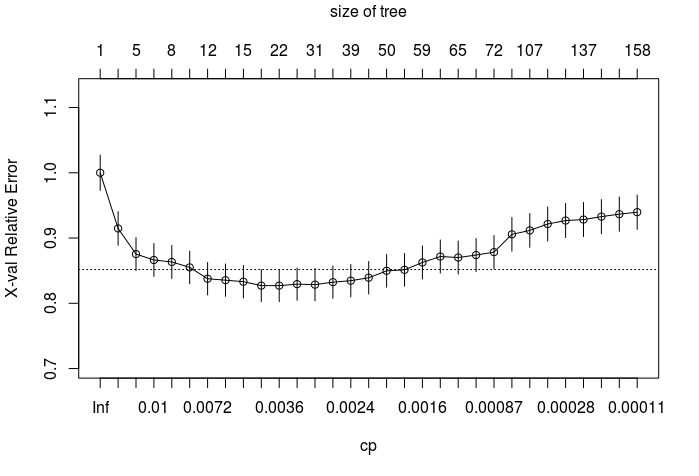
\includegraphics[width=0.5\textwidth]{graphics/cp.png}

	\caption{Evolution of xerror with increasing cp.}
\end{figure}

The best \textit{cp} is the one which minimises \textit{xerror}: $bestcp=0.00378$. After the pruning, the graph is smaller and more readable:

\begin{figure}[h]
	\centering

	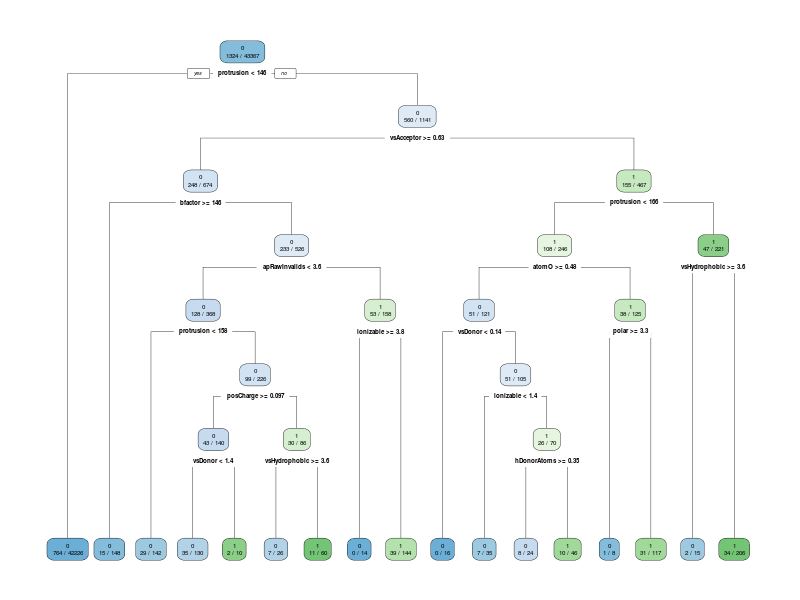
\includegraphics[width=0.45\textwidth]{graphics/tree.png}

	\caption{Decision tree graph. Green areas denote decisions with high confidence.}
\end{figure}

Such tree model will return confusion matrix for testing data (6633 rows) as follows:

\begin{center}
	\begin{tabular}{c|c|c c|}
	    \textbf{Confusion}  & & \multicolumn{2}{|c|}{\textbf{Prediction}} \\
		\hline
		  & & "No" & "Yes"\\
		\hline
		\multirow{2}{4em}{\textbf{Truth}} & "No" & ? & ? \\
		  & "Yes" & ? & ? \\
		\hline
	\end{tabular}
\end{center}

The mean accuracy according to cross-validation is around: \textbf{$97.09\%$}, which is quite worse, than Naive classifier. Usually, such instance-biased decision tree tends to overfit traning data and the performing lower generalisation ability.

\subsection{T-tests of DT model}

Cross-validation returned 10 results of accuracies following (at least we believe) normal distribution. After performing Student's t-tests, we obtained error intervals for the true mean accuracy of confidence $90\%$, $95\%$, $99\%$:

\begin{center}
	\begin{tabular}{c|c|c|c|}
    	  & \multicolumn{3}{|c|}{\textbf{Confidences}} \\
		\hline
		? & 90\% & 95\% & 99\% \\
		\hline
		? & ? & ? & ? \\
		\hline
	\end{tabular}
\end{center}

\subsection{Analysis of DT graph}

The DT graph on the left is not much readable, but provides at least some information about feature importance. The first big decision comes from the magnitude of \textit{protrusion}. If $protrusion < 146$, there is only $764/42226=1.8\%$ error of classifying protein point as inactive. In other case there comes second decision about \textit{vsAcceptor}, and so on. According to tree, one can identify several attributes as promising model features: protrusion, vsAcceptor, bfactor, vsHydrophobic,... Next model will tell more.

\newpage

%%%%%%%%%%%%%%%%%%%%%%%%%%%%%%%%%%%%%%%%%%%%%%%%%%%%%%%%%%%%%%%%%%%%%%%%%%%%%%%%%%%
\section{Model 2: Random Forest}

Second model is an ensemble model operating on multitude of decision trees, outputing the mode of the classes. As first, Random forest was trained with default settings. The OOB error (out-of-bag error) descreases with increasing number of used trees:

\begin{figure}[h]
	\centering

	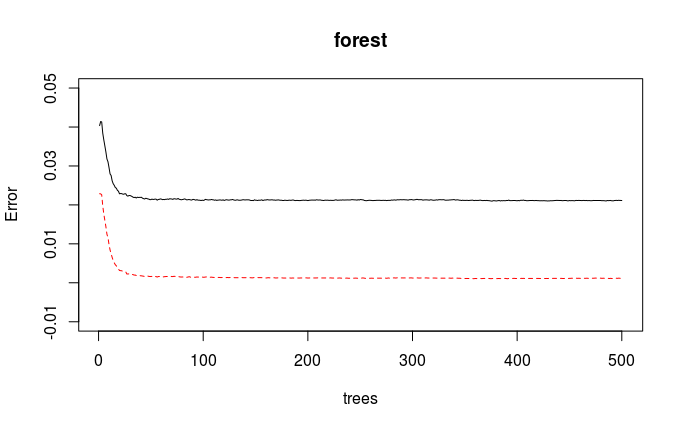
\includegraphics[width=0.5\textwidth]{graphics/forest-error.png}

	\caption{Black line: OOB error. Red line: one of class' error.}
\end{figure}

Second step is the tuning of parameter \textit{mtry}, which is standing for number of features used on each break. This was tested with smaller sample:

\begin{figure}[h]
	\centering

	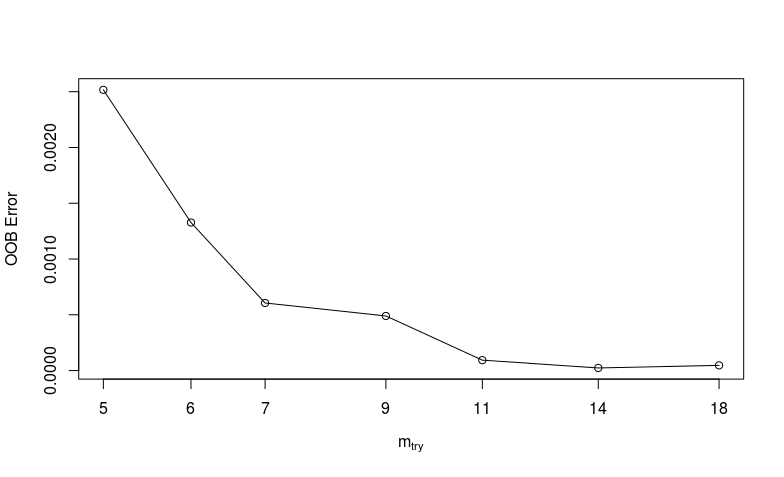
\includegraphics[width=0.5\textwidth]{graphics/OOB.png}

	\caption{CP}
\end{figure}

It looks like \textit{mtry} around 14 is good enough.

Confusion table for pruned random forest:

\begin{center}
	\begin{tabular}{c|c|c c|}
	    \textbf{Table}  & & \multicolumn{2}{|c|}{\textbf{Prediction}} \\
		\hline
		  & & "No" & "Yes"\\
		\hline
		\multirow{2}{4em}{\textbf{True}} & "No" & ? & ? \\
		  & "Yes" & ? & ? \\
		\hline
	\end{tabular}
\end{center}

With accuracy: ...

After cross-validation with above setup:

\begin{center}
	\begin{tabular}{c|c|c|c|}
    	  & \multicolumn{3}{|c|}{\textbf{Confidences}} \\
		\hline
		? & 90\% & 95\% & 99\% \\
		\hline
		? & ? & ? & ? \\
		\hline
	\end{tabular}
\end{center}


Variable importance:

\begin{figure}[h]
	\centering

	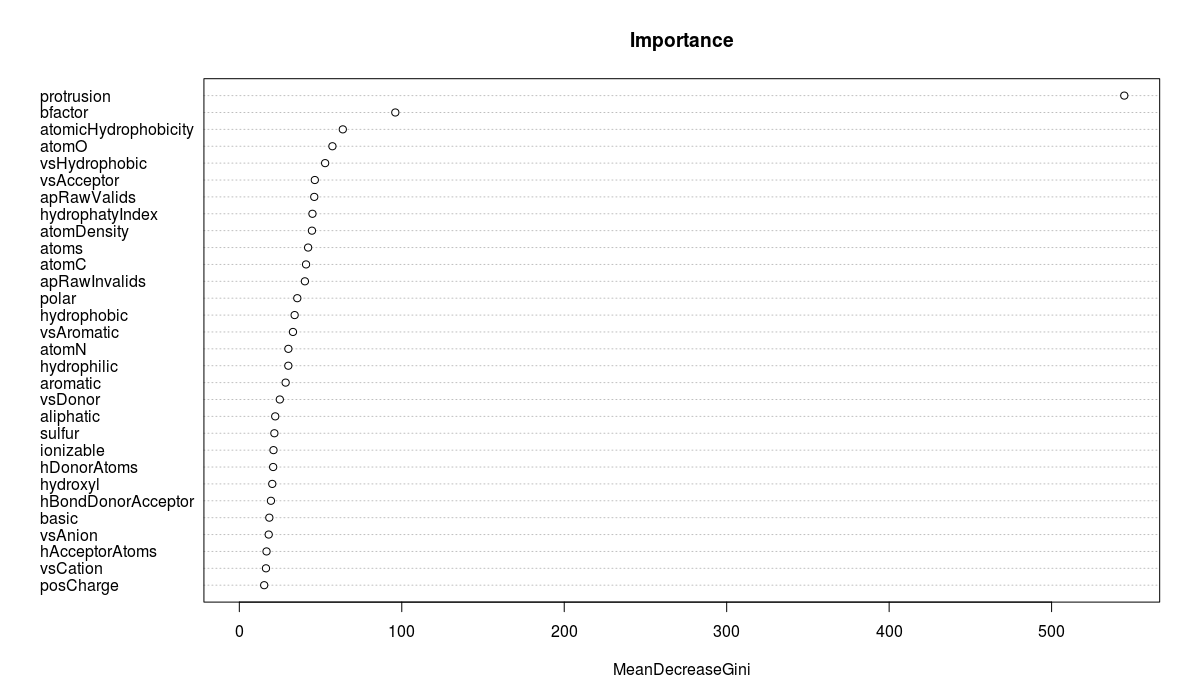
\includegraphics[width=0.5\textwidth]{graphics/importance.png}

	\caption{CP}
\end{figure}

\newpage
%%%%%%%%%%%%%%%%%%%%%%%%%%%%%%%%%%%%%%%%%%%%%%%%%%%%%%%%%%%%%%%%%%%%%%%%%%%%%%%%%%%

\section{Searching for feature set - SVM}

In this part I trained Support Vector Machine. First I tried linear, then polynomial model and then radial.

\subsection{Tuning SVM model}

Linear was shit, no better than naive. Polynomial of second order was better and radial one the best.

After this, I pruned the radial one for the best performance and the ran the cross-validation

\subsection{Forward selection}

Recall the feature diagram:

\begin{figure}[h]
	\centering

	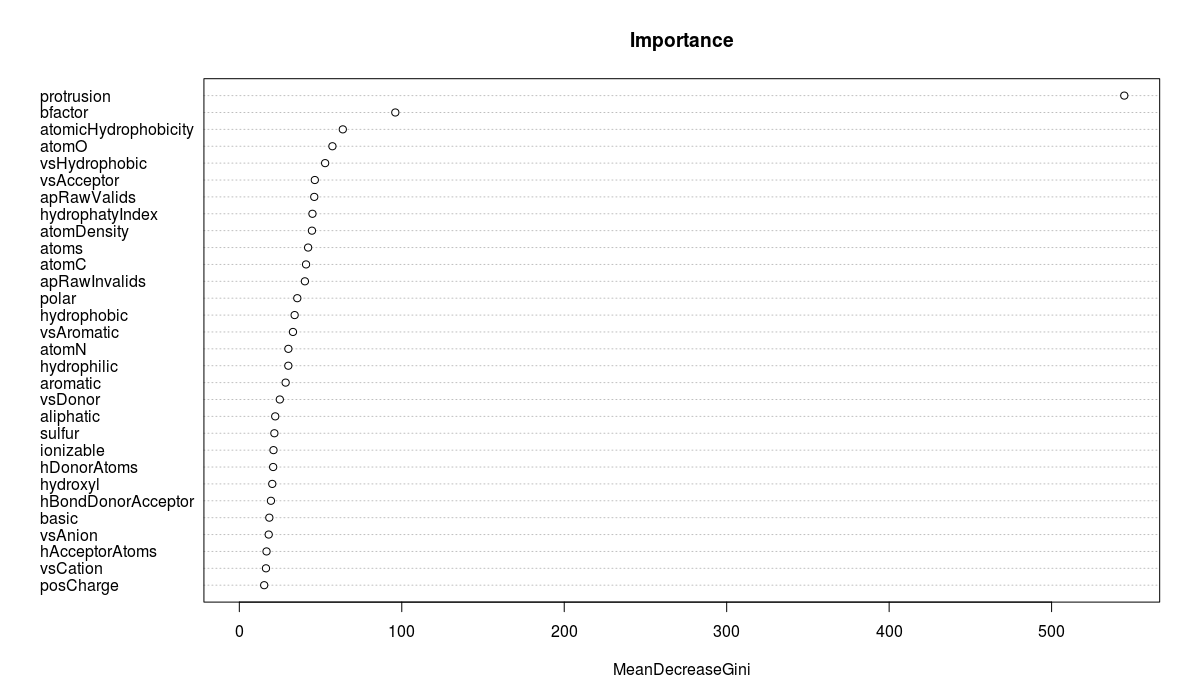
\includegraphics[width=0.5\textwidth]{graphics/importance.png}

	\caption{CP}
\end{figure}

Here I performed SVM model with radila kernel with feed-forwarding features.

Coming soon...


\newpage
%%%%%%%%%%%%%%%%%%%%%%%%%%%%%%%%%%%%%%%%%%%%%%%%%%%%%%%%%%%%%%%%%%%%%%%%%%%%%%%%%%%

\section{ROC evaluation}








\end{document}
%
% ****** End of file aipsamp.tex ******
